% @HEADER
% ***********************************************************************
%            MatrixPortal: A Web-Based Computing Environment
%
% Under terms of Contract DE-AC04-94AL85000, there is a non-exclusive
% license for use of this work by or on behalf of the U.S. Government.
%
% This library is free software; you can redistribute it and/or modify
% it under the terms of the GNU Lesser General Public License as
% published by the Free Software Foundation; either version 2.1 of the
% License, or (at your option) any later version.
%
% This library is distributed in the hope that it will be useful, but
% WITHOUT ANY WARRANTY; without even the implied warranty of
% MERCHANTABILITY or FITNESS FOR A PARTICULAR PURPOSE.  See the GNU
% Lesser General Public License for more details.
%
% You should have received a copy of the GNU Lesser General Public
% License along with this library; if not, write to the Free Software
% Foundation, Inc., 59 Temple Place, Suite 330, Boston, MA 02111-1307
% USA
% ***********************************************************************
% @HEADER

\documentclass[11pt,relax]{SANDreport}
\usepackage{graphicx}
\usepackage{amsmath,amsfonts,amsthm}
\usepackage{amssymb}
\usepackage{enumerate}
\usepackage{rotating}


\usepackage{times}

\def\choicebox#1#2{\noindent$\hphantom{th}$\parbox[t]{1.8in}{\sf
#1}\parbox[t]{4.5in}{#2}\\[0.8em]}

\author{Sala, Phenow, Hu, Tuminaro}

\title{On the Development of Portals for Scientific Computing (DRAFT)}
\SANDnum{SAND2006-XXXX}
\SANDauthor{Sala, Phenow, Hu, Tuminaro}

\SANDprintDate{July 2006}
\SANDreleaseType{Unlimited Release}

\newcommand{\Trilinos}{Trilinos}
\newcommand{\TrilinosTM}{Trilinos \copyright}
\newcommand{\trilinos}{{\sc Trilinos}}
\newcommand{\ifpack}{{\sc Ifpack}}
\newcommand{\aztecoo}{{\sc AztecOO}}
\newcommand{\amesos}{{\sc Amesos}}
\newcommand{\epetra}{{\sc Epetra}}
\newcommand{\ml}{{\sc ML}}
\newcommand{\mb}[1]{{\mathbf {#1} }}
\newcommand{\teuchos}{{\sc Teuchos}}
\newcommand{\triutils}{{\sc Triutils}}
\newcommand{\metis}{{\sc METIS}}

\newcommand{\ie}{i.e., }
\newtheorem{assumption}{Assumption}[section]
\newtheorem{lemma}{Lemma}[section]
\newtheorem{proposition}{Proposition}[section]
\newtheorem{corollary}{Corollary}[section]
\newtheorem{theorem}{Theorem}[section]
\newtheorem{algorithm}{Algorithm}[section]
\newtheorem{definition}{Definition}[section]
\newtheorem{property}{Property}[section]

\newtheorem{remark}{Remark}
\newtheorem{problem}{Problem}

\def\choicebox#1#2{\noindent$\hphantom{th}$\parbox[t]{3.0in}{\sf
#1}\parbox[t]{3.35in}{#2}\\[0.8em]}

\begin{document}

\maketitle

\begin{abstract}
Organizations have quickly realized the potential of Web Portals to foster and
promote the creation and reuse of knowledge. Many portal systems have been
developed to provide a gateway or launch pad to find and reutilize
information.

In this report, we apply the portal technology to the development and usage of
scientific software libraries.  We present a set of tools that can help to
evaluate the performances of scientific software, and in particular of linear
algebra libraries for high-performance computing. We present the design and
implementation of a  web interface that offers a widely accessible,
               homogeneous and easy-to-use graphical interface to a suite of
               linear algebra solvers.  This user-friendly interface promotes
               testing and experimenting with a variety of state-of-the-art
               linear algebra libraries for distributed sparse matrices.
\end{abstract}

\clearpage
\begin{center}
(page intentionally left blank)
\end{center}

\SANDmain

\tableofcontents

\clearpage
\newpage


% ------------------------------------------------------------------------- %
\section{Introduction}
% ------------------------------------------------------------------------- %

In the language of the World Wide Web (WWW), a {\sl portal}, or portal site,
is the site that users visit first. As its name stands for, it acts as a
doorway to all the resources of a given subject. Typically, a portal gives a
single, coherent view of information aggregated from disparate sources or
providers. 

Here, we are investigating the issues related to the development
and implementation of a portal for scientific computing. Therefore, we will
only consider {\sl vertical portal}, developed for a specified audience ---
that is, scientific computing. Although the ideas we present can in principle
be applied to a vast group of software projects, we will focus our attention
to sparse linear algebra.

MatrixPortal is intended to be a generic
toolkit that enables users to quickly test and get experience. The Web
interface encapsulates, in a high level of abstraction, the most prominent
features of the supported libraries. By offering a service like the
MatrixPortal, we hope to make our work
accessible to a larger target audience, and to receive feedback from the user
community.

We design our portal as a Web service. The Web Web standards have been
conceived to support interoperability, i.e., independence of the transport
protocols, programming languages, programming models, and system software.
Being based on industry standards like XML and HTML, a portal does not require
any special purpose hardware or software.  Since the services reside only on
the web server(s), the client software does not need to be updates every time
the web service is modified; changes to the interfaces simply need a "reload"
procedure.  The web service code never leaves the server, so property code is
protected. And, last but not least, Web services can be accessed from
everywhere and no special purpose interfaces are necessary.

\medskip

This report is organized as follows. Section~\ref{sec:design} presents the
design requirements and objectives of the portal.
Section~\ref{sec:navigation} outlines the navigation model.  The computational
model is described in Section~\ref{sec:computational}. A concrete
implementation is outlines in Section~\ref{sec:concrete}.  Finally,
               Section~\ref{sec:concluding} reports the conclusions and the
               future works.

% ------------------------------------------------------------------------- %
\section{Design Models for Scientific Computing Portals}
\label{sec:design}
% ------------------------------------------------------------------------- %

Initially, the term portal was used to refer to Internet search and navigation
sites that provide a starting point to explore the Web. Portals have now
reached a certain maturity, and can now be divided into {\sl horizontal} and
{\sl vertical} portals. Horizontal portals target the entire Internet
community. These sites usually contain search engines and provide the ability
for user to personalize the page. A vertical portal, instead, are customized
to niche audiences about a particular area of interest. As such, vertical
portals offer access to specialized information. We are in particular
interested in two types of vertical portals: {\sl workspace portals} and {\sl
knowledge portals}. The firmat offer a single, coherent, integrated
environment that presents its users with all the information they need to
carry out their jobs. Knowledge portals, instead, aim to increase the
effectiveness of knowledge workers by providing easy access to information
that is necessary or helpful to them to carry out their jobs. 

These concepts can be applied to the development and usage of scientific
libraries as follows. Knowledge portals are portals for a novice user. They
are developed to minimize the investment
from this (casual) user, as well as the time required to move from the problem
specification to the data analysis. A possible usage of the novice mode is for
live presentations, or for teaching purposes. Novice portals as a simple view
of a complex world.

Workspace portals, instead, will be built to offer a large set of
functionalities. In expert mode, the portal can be used as a scientific
computational tool, where real-life problems can be solved, and the solution
can be post-processed or sent to the user.  A key point to note in this
category is the issue of trust. Typically, expert users can upload their own
problems, and possibly define a custom script of compilation file. To avoid
abuses or misuses of the system, only certified users can receive the
authorizations to access this expert mode.

\bigskip

MUST LOOK HERE: \verb!http://tyne.dl.ac.uk/GROWL/portal_guide/node3.html!

Talk about SANS (Self-Adapting Numerical Software)??? What else???

\verb!http://esc.dl.ac.uk/HPCPortal/!

Basic grid portal computing 
EPCC MHD portal, HPCGrid Portal 
Advance portal computing 
ASC Portal (Cactus Portal) 
Small scale grids (LSF, PBS, Condor) 
Toolkit approach (Globus, Legion, Unicore) 
Internet computing (Entropia, SETI@home)and peer-to-peer computing (Napster, Gnutella etc.)


www.gridforum.org

www.gridlab.org 

www.epcc.ed.ac.uk/ENACTS/

% ------------------------------------------------------------------------- %
\subsection{Portal Objectives}
% ------------------------------------------------------------------------- %

Why are portals needed in the field of scientific computing? In
our opinion, the following motivations suggest that such a project could
benefit the research community:
\begin{itemize}
\setlength{\itemsep}{0pt}
\item Scientific libraries can require quite different amount
of knowledge to be unleashed. Software projects are sometimes large, and the
learning curve can be steep. Typically, it is not easy for the intended user
to load up his or her data and solve the corresponding problem with a new
library. This can slow down the testing, usage and acceptance of new 
projects. Being language-independent, and with no need to download or install
any software, a portal offers a demo version of the actual library, whose
usage only requires a small amount of data from the user, or no data at all if
a problem generator is selected.
%
\item For teaching and learning purposes, it can be of interest to move
smoothly from theoretical results to practical evidence.
Users interested only in the specific results 
(e.g., the iterations to converge for a given preconditioner) could benefit
from pop-down menus and common test problems.
%
\item By using a portal,
the need to configure, compile and install is lifted. These steps are
generally challenging  for
the unexperienced user, and a time-consuming step for both unexperienced and
expert users. Besides, some configuration options may require additional
libraries.
%
\item Bug-tracking capabilities like Bugzilla~\cite{bugzilla} and mailing
lists help to create a sense of community, they are often not effective enough
to share data. A web portal can improve the communication between users and
developers and among users: if a certain bug can be reproduced on the portal,
           then developers will have all required data and access to the buggy
           code. Equivalently, users can share tricks or solutions. This can
           be a step forward {\sl collaborative computing}.
%
\item Comparing different versions, or compare the installed version with the
latest can become as easy as selecting one option in a list. Then, the user
can decide whether the new version deserves to be downloaded and installed or
not.
\end{itemize}

% ------------------------------------------------------------------------- %
\subsection{Portal Requirements}
% ------------------------------------------------------------------------- %

We divide the requirements in two groups: those for users and those for
portal developers. 

In the former group we include {\sl flexibility}, {\sl scalability} and {\sl
  low latency}. Obviously, the greatest investment goes to the user interface.
We are interesting in a user interface that favors the
experimentation process, and offer an extensive list of parameters to toggle
the behavior of the solvers, as well as a detailed help to guide users with
less experience. The main requirement here is for a clean and uniform design,
which avoids
everything that can be misinterpreted or can lead to confusion. The user
should be able to assign custom names to problem definitions, and perform 
a valid performance analysis. Performance analysis is required to help the 
decision-making processing for the user's application.  Conveying the
results in a clear and understandable way is a major objective of our work.

The requirements for portal developers are centered around 
{\sl extensibility}.  
The design philosophy is that of a ``bag of services,'' that is, we aim to
offer a variety of solutions for a given problem. A user interested in using
the portal does not have to adopt any particular programming model or
language, to learn or read any documentation or to configure and install any
software. This means that 
only a minimal investment should be required to add new
capabilities, like supporting a new package or adding a new drop-down menu.
{\sl Security} issues should not be underestimated. 

% ------------------------------------------------------------------------- %
\section{The Portal from the User's Perspective}
\label{sec:navigation}
% ------------------------------------------------------------------------- %

% ------------------------------------------------------------------------- %
\subsection{Novice Mode}
% ------------------------------------------------------------------------- %

\begin{figure}
\begin{center}
\begin{tabular}{c c c}
%
\begin{tabular}{| p{3.5cm} |}
\hline \\ Setup problems \\  \\ \hline
\end{tabular} 
& $\Rightarrow$ & 
%
\begin{tabular}{| p{3.5cm} |}
\hline \\ Analyze data\\ \\ \hline
\end{tabular}  \\
% - newline - %
               &               & $\Downarrow$ \\
% - newline - %
\begin{tabular}{| p{3.5cm} |}
\hline \\ Save results in XML\\ \\ \hline
\end{tabular}  
&  &
\begin{tabular}{| p{3.5cm} |}
\hline \\ Specify parameters\\ \\ \hline
\end{tabular}  \\
% - newline - %
$\Uparrow$     &               &    $\Downarrow$ \\
% - newline - %
\begin{tabular}{| p{3.5cm} |}
\hline \\ Analyze data\\ \\ \hline
\end{tabular}  & $\Leftarrow$ &
\begin{tabular}{| p{3.5cm} |}
\hline \\ Compute solutions\\ \\ \hline
\end{tabular}  \\
\end{tabular}
\end{center}
\caption{}
\label{fig:navigation}
\end{figure}

The navigation of the web portal in the novice mode is reported in
Figure~\ref{fig:navigation}. 
We now analyze in more details these phases. First, the user has to specify
the linear system to be solved. The easiest way for doing this is to use a
data generation tool, thus creating data on-the-fly. This is equivalent to
using the {\tt gallery} function of MATLAB\copyright. Authorized users can
also upload their data. This requires a standard data format. We adopt both
the well-known Harwell-Boeing format, and the XML-based format furnished by
the EpetraExt package of Trilinos. Then, some basic checks on the selected
data is performed. The next phase is the specification of the solution
parameters, followed by the actual solution of the linear systems. The output
is sent to the user's Web browser, where the evaluation phase can be
performed. The evaluation step allows to classify the solvers depending on
quantitative information like the iterations to converge, the CPU time
required for the solution, or the condition number.  Simple graphical tools
are offered to help the decision making.

We aim to minimize the vocabulary required to use a given library. A clear
understanding of a software project requires agreement on standard terms.

% ------------------------------------------------------------------------- %
\subsection{Expert Mode}
% ------------------------------------------------------------------------- %

Navigation in expert mode is pretty simple: users have to write their own
scripts, or cut-and-paste it, then click on the appropriate button to start
the automatic compilation and execution. Depending on the configuration,
serial or parallel, MPI-based computations is performed. A collection of code
fragments and complete examples is made available to speed up the writing
phase.

Working with the portal in expert mode can shorted the learning curve, since
no software has to be downloaded, configured, compiled and installed. Also,
all the appropriate compilation flags have already been selected -- and the
users do not need to read and understand any manuals or documentation.
However, the expert mode currently has several limitations. First, the editing
occurs on a \verb!textarea! box, with limited editing capabilities compared to
tools like \verb!emacs! or \verb!vi!. Second, the program cannot be executed
through a debugger, and only its final output (plus possibly the stack trace
                                               in the case of a core dump) is
available. The current configuration does not allow to include more than one
file, or to save the file on the server, nor it is possible to link against
libraries that are not automatically supported by the portal compilation tool.

Considering these limitations, the portal in expert mode should be used mostly
for {\sl self-learning} purposes. If shipped with a rich collection of
scripts and extensive help, it can shorten the time required by a new user to
get a basic knowledge of a software project. That is, it acts as a {\sl demo
version}, freely available with minimal investment to the interested user.
If convinced by the utility of the project, then the user can start the
download/configure/compile/install cycle required to fully take advantage of
the project. Another important usage is {\sl teaching}. Hands-on sessions can
be quickly organized without installing any software on all the computers in
the classroom --- a long and error-prone operation.

% ------------------------------------------------------------------------- %
\section{The Portal from the Server's Perspective}
\label{sec:computational}
% ------------------------------------------------------------------------- %

Section~\ref{sec:navigation} has shown the portal from the user's perspective.
This section describes the models that makes all of this possible, easily
configurable, and portal on almost all web servers.

We structure the portal as a client-server structure. 
An overview of the structure is reported in Figure~\ref{fig:design}.
The client side is the
user's interface described in the previous section, and it is 
basically composed by a Web browser, and possibly
authentication tools. The server side, or back-end, is composed by 
the {\sl portal server} that interacts with the client and transmit Web pages,
a {\sl certified server} to upload and download data (data repository), and the {\sl computing
  resources}. These three components can be located on the same physical
  machine, or being distributed. In this latter case we have a
  client-server-solver model. Note that the data repository might require
intensive exchange through the network. 

\begin{figure}
\begin{center}
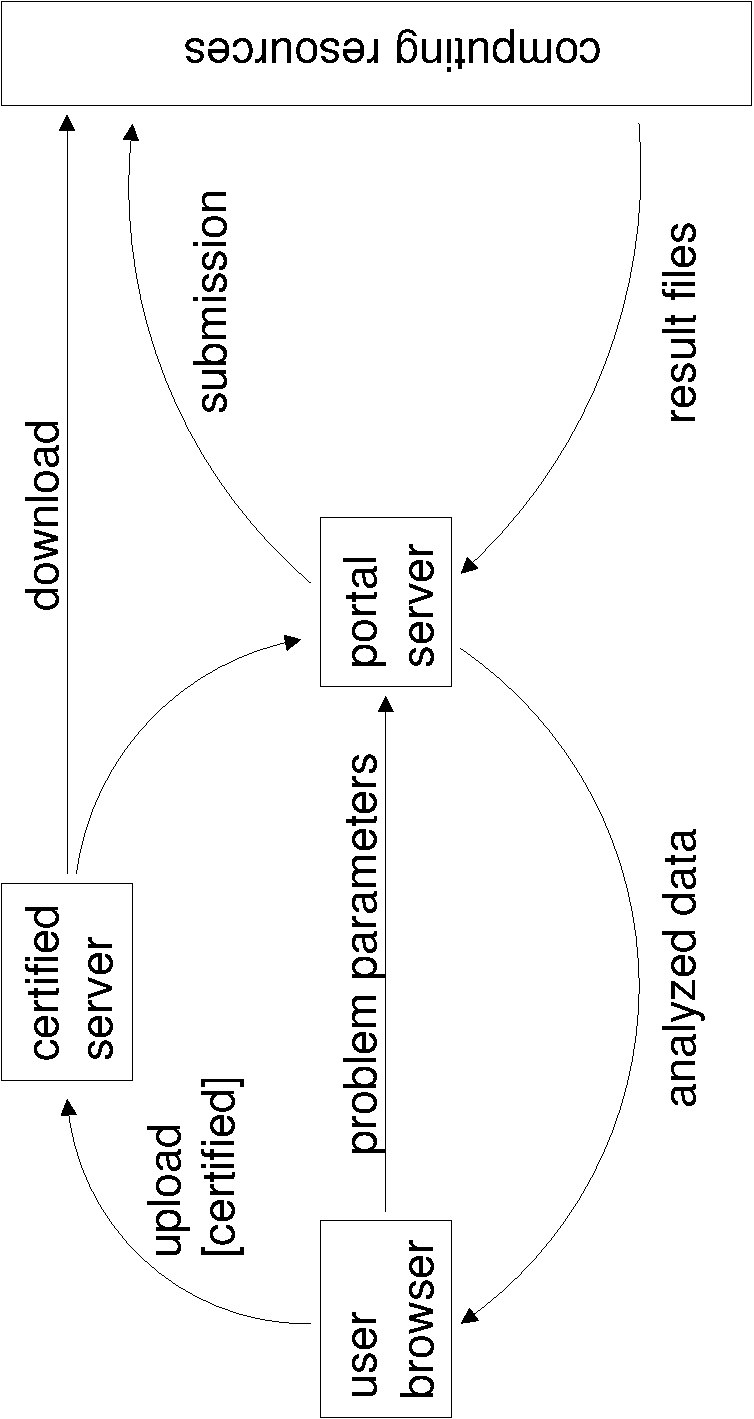
\includegraphics[width=14cm]{portal_design}
\caption{Design}
\end{center}
\label{fig:design}
\end{figure}

% ------------------------------------------------------------------------- %
\section{A Concrete Implementation}
\label{sec:concrete}
% ------------------------------------------------------------------------- %

With the term {\sl portal for scientific computing} we mean a web-based
interface to access high-performance software libraries. Among several
possible choices, we consider the Trilinos project~\cite{trilinos}
as concrete implementation
of our model. However, other projects (like PETSc~\cite{petsc-guide} 
                                       or Hypre~\cite{hypre}) could
straightforwardly be included in our portal.

The current architecture of MatrixPortal is designed to support both the
novice and expert usage.
The portal is based on commodity Web technologies,
and it can be run by anyone who has access to a Web browser with support for
HTML 3.0, JavaScript 1.1, and the SSL protocol.  No special plugins are
required, nor a Java machine is used. This increases its portability.

From the server's perspective, our implementation requires:
\begin{itemize}
\item a Web server (like Apache) with support for PHP version 4 or more recent;
\item Python version 2.4 or more recent;
\item Scientific libraries like BLAS and LAPACK, and possibly METIS and
ParMETIS;
\item Trilinos 7.0 or more recent. 
In particular, we use the Python interface to Trilinos, PyTrilinos.
\end{itemize}
The implementation diagram is reported in Figure~\ref{fig:design}.
\begin{figure}
\begin{center}
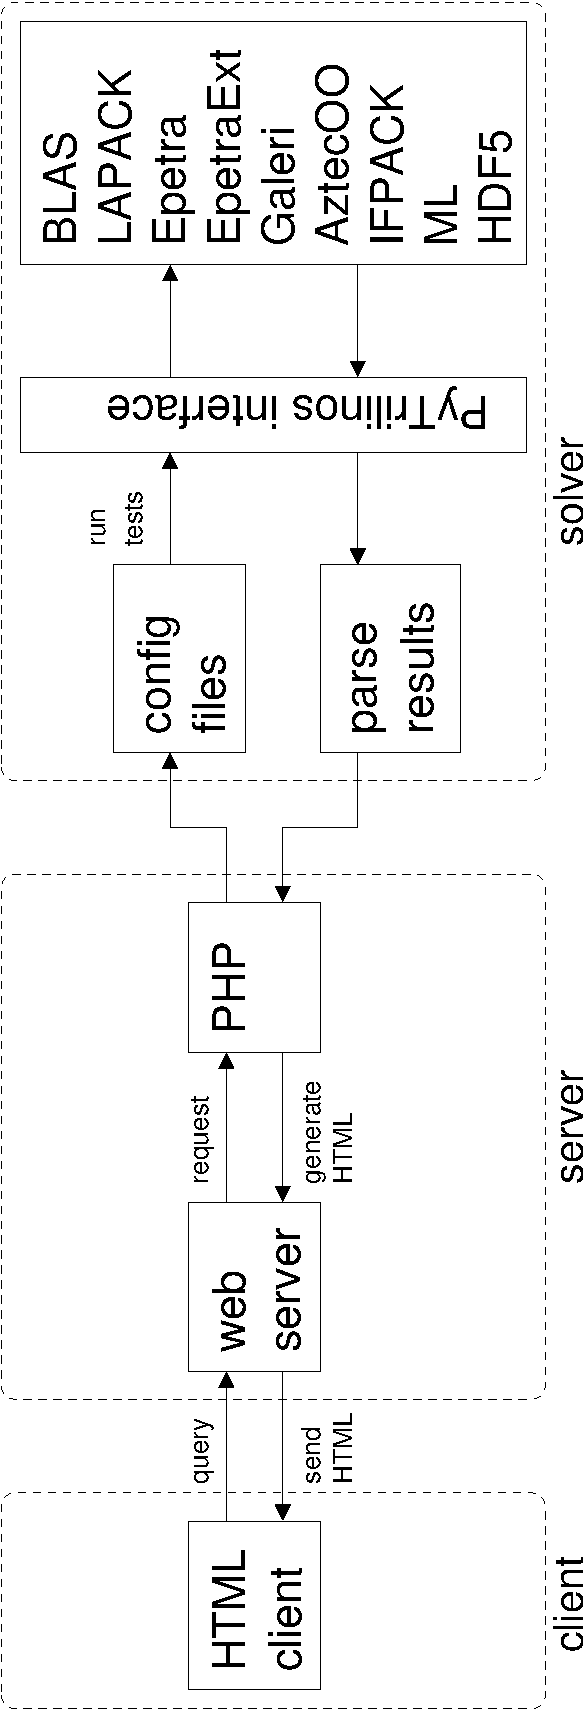
\includegraphics[width=14cm]{diagram}
\caption{Implementation diagram.}
\label{fig:design}
\end{center}
\end{figure}

% ------------------------------------------------------------------------- %
\section{Concluding Remarks}
\label{sec:concluding}
% ------------------------------------------------------------------------- %

We have described the design issues for a portal targeted to scientific
computing, with particular emphasis on sparse linear algebra. Motivations for
creating web portals are to ease experimentation, increase communication
between users and developers and within developers, scientific computation,
        and teaching. The described portal 
eases exploring new strategies with minimal investment and allows the
casual user to explore the algorithms and ideas offered by a scientific
library, and not by the implementation and installation details.
The advantages are:
1) The researcher can study the system, learn about the state-of-the-art, and
generate theories from practice. 2) The researcher can answer ``how'' and
``why'' questions to gain a better understanding of the processes taking
place. 3) The researcher can investigate an area in which few previous studies
have been carried out.

% ------------------------------------------------------------------------- %
\section*{Acknowledgments}
% ------------------------------------------------------------------------- %


% ------------------------------------------------------------------------- %
\bibliographystyle{plain}
\bibliography{biblio}
% ------------------------------------------------------------------------- %

\end{document}
